\documentclass[journal,onecolumn]{vgtc}                     % final (journal style)
%\documentclass[journal,hideappendix]{vgtc}        % final (journal style) without appendices
%\documentclass[review,journal]{vgtc}              % review (journal style)
%\documentclass[review,journal,hideappendix]{vgtc} % review (journal style)
%\documentclass[widereview]{vgtc}                  % wide-spaced review
%\documentclass[preprint,journal]{vgtc}            % preprint (journal style)


%% Uncomment one of the lines above depending on where your paper is
%% in the conference process. ``review'' and ``widereview'' are for review
%% submission, ``preprint'' is for pre-publication in an open access repository,
%% and the final version doesn't use a specific qualifier.

%% If you are submitting a paper to a conference for review with a double
%% blind reviewing process, please use one of the ``review'' options and replace the value ``0'' below with your
%% OnlineID. Otherwise, you may safely leave it at ``0''.
\onlineid{0}

%% In preprint mode you may define your own headline. If not, the default IEEE copyright message will appear in preprint mode.
%\preprinttext{To appear in IEEE Transactions on Visualization and Computer Graphics.}

%% In preprint mode, this adds a link to the version of the paper on IEEEXplore
%% Uncomment this line when you produce a preprint version of the article
%% after the article receives a DOI for the paper from IEEE
%\ieeedoi{xx.xxxx/TVCG.201x.xxxxxxx}

%% declare the category of your paper, only shown in review mode
\vgtccategory{Research}

%% please declare the paper type of your paper to help reviewers, only shown in review mode
%% choices:
%% * algorithm/technique
%% * application/design study
%% * evaluation
%% * system
%% * theory/model
\vgtcpapertype{application/design study}

%% Paper title.
\title{Details of Computation}

%% Author ORCID IDs should be specified using \authororcid like below inside
%% of the \author command. ORCID IDs can be registered at https://orcid.org/.
%% Include only the 16-digit dashed ID.
\author{%
  \texorpdfstring{Stephen Jasina, Loqman Salamatian, Joshua Mathews, Scott Anderson, \\ Paul Barford, Mark Crovella, and Walter Willinger}{Stephen Jasina, Loqman Salamatian, Joshua Mathews, Scott Anderson, Paul Barford, Mark Crovella, and Walter Willinger}
}

% \authorfooter{
%   %% insert punctuation at end of each item
%   \item
%   	Josiah Carberry is with Brown University.
%   	E-mail: jcarberry@example.com
%   \item
% }

%% Abstract section.
% \abstract{}

%% Keywords that describe your work. Will show as 'Index Terms' in journal
%% please capitalize first letter and insert punctuation after last keyword
% \keywords{}

%% Uncomment below to disable the manuscript note
% \renewcommand{\manuscriptnotetxt}{}

%% Copyright space is enabled by default as required by guidelines.
%% It is disabled by the 'review' option or via the following command:
%\nocopyrightspace


%%%%%%%%%%%%%%%%%%%%%%%%%%%%%%%%%%%%%%%%%%%%%%%%%%%%%%%%%%%%%%%%
%%%%%%%%%%%%%%%%%%%%%% LOAD PACKAGES %%%%%%%%%%%%%%%%%%%%%%%%%%%
%%%%%%%%%%%%%%%%%%%%%%%%%%%%%%%%%%%%%%%%%%%%%%%%%%%%%%%%%%%%%%%%

%% Tell graphicx where to find files for figures when calling \includegraphics.
%% Note that due to the \DeclareGraphicsExtensions{} call it is no longer necessary
%% to provide the the path and extension of a graphics file:
%% 
\includegraphics{diamondrule} is completely sufficient.
\graphicspath{{figs/}{figures/}{pictures/}{images/}{./}} % where to search for the images

\usepackage{amsfonts, amsmath, amssymb, amsthm}
\usepackage[svgnames]{xcolor}
\usepackage{tikz}

%% We encourage the use of mathptmx for consistent usage of times font
%% throughout the proceedings. However, if you encounter conflicts
%% with other math-related packages, you may want to disable it.
\usepackage{mathptmx}                  % use matching math font

\allowdisplaybreaks

\delimitershortfall-1pt

\newcommand*\delimeter[3]{
	\ensuremath{\mathopen{}\left#2 #1\right#3\mathclose{}{\vphantom{\left#2 #1\right#3}}}
}

\newcommand*\pof[1]{\delimeter{#1}{(}{)}}
\newcommand*\plof[1]{\delimeter{#1}{(}{.}}
\newcommand*\prof[1]{\delimeter{#1}{.}{)}}
\newcommand*\sof[1]{\delimeter{#1}{[}{]}}
\newcommand*\slof[1]{\delimeter{#1}{[}{.}}
\newcommand*\srof[1]{\delimeter{#1}{.}{]}}
\newcommand*\cof[1]{\delimeter{#1}{\{}{\}}}
\newcommand*\clof[1]{\delimeter{#1}{\{}{.}}
\newcommand*\crof[1]{\delimeter{#1}{.}{\}}}
\newcommand*\aof[1]{\delimeter{#1}{\langle}{\rangle}}
\newcommand*\alof[1]{\delimeter{#1}{\langle}{.}}
\newcommand*\arof[1]{\delimeter{#1}{.}{\rangle}}

\newcommand*\abs[1]{\delimeter{#1}{|}{|}}
\newcommand*\norm[1]{\delimeter{#1}{\|}{\|}}
\newcommand*\floor[1]{\delimeter{#1}{\lfloor}{\rfloor}}
\newcommand*\ceil[1]{\delimeter{#1}{\lceil}{\rceil}}

\newcommand*\ooint[1]{\delimeter{#1}{(}{)}}
\newcommand*\ocint[1]{\delimeter{#1}{(}{]}}
\newcommand*\coint[1]{\delimeter{#1}{[}{)}}
\newcommand*\ccint[1]{\delimeter{#1}{[}{]}}

\newcommand*\eval[1]{\delimeter{#1}{.}{|}}

\newcommand*\Dif{\ensuremath{\mathrm{D}}}
\newcommand*\dif{\ensuremath{\mathrm{d}}}


\DeclareMathOperator{\proj}{proj}
\DeclareMathOperator{\sgn}{sgn}

\DeclareMathOperator{\GCL}{GCL}
\DeclareMathOperator{\RTT}{RTT}

\DeclareMathOperator{\nxt}{nxt}

\begin{document}
	\maketitle

	This document details the strategy for computing important quantities on a mesh, like curvature, as well as the loss functions based on these quantities. Furthermore, details of computing gradients of these quantities are presented.

	Due to the necessity of much more notation than in the main paper, some choices of letters will differ.

	\subsection{Inputs and Outputs}
As input to the optimization process, we take an weighted undirected graph \(G = \pof{V_G, E_G}\). Each vertex \(s \in V_G\) represents a node in a network and is annotated with location information. We therefore can compute quantities like \(\GCL\pof{s, s'}\), the Great Circle Latency between \(s\) and \(s'\).

Additionally, an edge \(\cof{s, s'} \in E_G\) has an associated measured Round Trip Time \(\RTT\pof{s, s'}\). In practice, latencies are collected for almost every pair of nodes, so \(G\) is nearly complete.

We also take several hyperparameters. First is the residual latency threshold \(\epsilon\). Next are the \(\lambda\)'s, which are weighting parameters for each component of the loss function. Finally, there are a few hyperparameters describing the structure of the mesh.

We return a triangle mesh \(M = \pof{V_M, E_M}\), stored in a doubly connected edge list format. That is, each edge is actually stored as a pair of directed edges, except for on the boundary, where only a single directed edge is used. These directed edges trace out each face of the mesh counterclockwise.

As hinted at above, the actual vertex-edge connectivity of the mesh is to be selected before running the optimization. That said, each vertex has coordinates in \(\mathbb{R}^3\) which are to be chosen by the optimization algorithm. For the purposes of the algorithm and mesh regularity, we parameterize each vertex position with a single number. In our current implementation, each vertex \(v \in V_M\) can be broken into parts as \(\pof{p_v, z_v}\), where \(p_v\) is a latitude-longitude pair, and \(z_v\) is an altitude. The optimization algorithm then determines the best \(z\) values.

Note that the above parameterization implies we can map vertices \(s \in V_G\) to positions on the mesh \(\pi\pof{s}\). For the purposes of the following computations, assume the stronger statement \(\pi\pof{s} \in V_M\). While this assumption is not strictly necessary, it significantly simplifies the geodesic distance computation. Furthermore, provided our mesh is fine enough, the stronger assumption will lead to minimal numerical error.


	\subsection{Laplacian}

Here and in the subsequent sections, computations can take serious advantage of vectors and matrices. Therefore, while notationally inelegant, we will assign indices to the vertices in \(V_M\).

On that note, if \(i\) and \(j\) are two indices for which \(\pof{v_i, v_j} \in E_M\), let \(\nxt\pof{i, j}\) be the index such that \(v_i \to v_j \to v_{\nxt\pof{i, j}}\) traces a triangle counterclockwise. If \(\nxt\pof{i, j}\) does not exist, then the half-edge \(\pof{v_i, v_j}\) lies on the boundary.

We also write \(\partial M\) to represent the boundary of our mesh. Abusing notation, we can write \(v_i \in \partial M\) and \(\pof{v_i, v_j} \in \partial M\) to denote that a vertex or an edge is on the boundary, respectively.

In this and the following sections, we will lay out what each variable is before the details of computing it. We also give the (total) runtime in big-\(O\) notation to compute the set of variables and its gradients. For the Laplacian, we have:

\begin{figure*}[h!]
    \centering
    \begin{tabular}{r|l|l}
    	\(N_{i, j}\) & Outward normal of triangle \(v_i \to v_j \to v_{\nxt\pof{i, j}}\) & \(O\pof{\abs{V_M}}\) \\ \hline
    	\(A_{i, j}\) & Area of triangle \(v_i \to v_j \to v_{\nxt\pof{i, j}}\) & \(O\pof{\abs{V_M}}\) \\ \hline
    	\(D_{i, j}\) & Vertex triangle areas; diagonal & \(O\pof{\abs{V_M}}\) \\ \hline
    	\(\theta_{i, j}\) & Measure of \(\angle v_iv_{\nxt\pof{i, j}}v_j\) & \(O\pof{\abs{V_M}}\) \\ \hline
    	\(L_C^{\text{N}}\) & Cotangent operator with zero-Neumann boundary condition & \(O\pof{\abs{V_M}}\) \\ \hline
    	\(L_C^{\text{D}}\) & Cotangent operator with zero-Dirichlet boundary condition & \(O\pof{\abs{V_M}}\)
    \end{tabular}
    \captionsetup{labelformat=empty}\caption{}
\end{figure*}

\subsubsection{Forward Computation}
We have the following (standard) definition of the Laplace-Beltrami operator on a mesh:

\begin{align*}
	N_{i, j} &= \pof{v_i - v_{\nxt\pof{i, j}}} \times \pof{v_j - v_{\nxt\pof{i, j}}}, \\
	A_{i, j} &= \frac{1}{2}\norm{N_{i, j}}_2, \\
	D_{i, j} &= \begin{cases}
		\frac{1}{3}{\displaystyle\sum_{\substack{k \\ \pof{v_i, v_k} \in E_M}}A_{i, k}} & \text{if \(i = j\)}, \\
		0 & \text{otherwise},
	\end{cases} \\
	\cot\pof{\theta_{i, j}} &= \frac{\pof{v_i - v_{\nxt\pof{i, j}}} \cdot \pof{v_j - v_{\nxt\pof{i, j}}}}{2A_{i, j}}, \\
	\pof{L_C^{\text{N}}}_{i, j} &= \begin{cases}
		\frac{1}{2}\cot\pof{\theta_{i, j}} & \text{if \(\pof{v_i, v_j} \in \partial M\)}, \\
		\frac{1}{2}\cot\pof{\theta_{j, i}} & \text{if \(\pof{v_j, v_i} \in \partial M\)}, \\
		\frac{1}{2}\pof{\cot\pof{\theta_{i, j}} + \cot\pof{\theta_{j, i}}} & \text{if \(\pof{v_i, v_j}, \pof{v_j, v_i} \in E_M\)}, \\
		-\frac{1}{2}\pof{\displaystyle\sum_{\substack{k \\ \pof{v_i, v_k} \in E_M}}\cot\pof{\theta_{i, k}} + \sum_{\substack{k \\ \pof{v_k, v_i} \in E_M}}\cot\pof{\theta_{k, i}}} & \text{if \(i = j\)}, \\
		0 & \text{otherwise},
	\end{cases} \\
	\pof{L_C^{\text{D}}}_{i, j} &= \begin{cases}
		\frac{1}{2}\pof{\cot\pof{\theta_{i, j}} + \cot\pof{\theta_{j, i}}} & \text{if \(\pof{v_i, v_j} \in E_M\), \(v_i \not\in \partial M\), and \(v_j \not\in \partial M\)}, \\
		-\frac{1}{2}{\displaystyle\sum_{\substack{k \not\in \partial M \\ \pof{v_i, v_k} \in E_M \\ \pof{v_k, v_i} \in E_M}}\pof{\cot\pof{\theta_{i, k}} + \cot\pof{\theta_{k, i}}}} & \text{if \(i = j\) and \(v_i \not\in \partial M\)}, \\
		0 & \text{otherwise}.
	\end{cases}
\end{align*}

\subsubsection{Reverse Computation}
We compute

\begin{align*}
	\frac{\partial v_i}{\partial z_\ell} &= \begin{cases}
		e_3 & \text{if \(\ell = i\)}, \\
		0 & \text{otherwise},
	\end{cases} \\
	\frac{\partial N_{i, j}}{\partial z_\ell} &= \begin{cases}
		\pof{v_{\nxt\pof{i, j}} - v_j} \times \frac{\partial v_\ell}{\partial z_\ell} & \text{if \(\ell = i\)}, \\
		\pof{v_i - v_{\nxt\pof{i, j}}} \times \frac{\partial v_\ell}{\partial z_\ell} & \text{if \(\ell = j\)}, \\
		\pof{v_j - v_i} \times \frac{\partial v_\ell}{\partial z_\ell} & \text{if \(\ell = \nxt\pof{i, j}\)}, \\
		0 & \text{otherwise},
	\end{cases} \\
	\frac{\partial A_{i, j}}{\partial z_\ell} &= \frac{1}{4A_{i, j}}N_{i, j} \cdot \frac{\partial N_{i, j}}{\partial z_\ell}, \\
	\pof{\frac{\partial D}{\partial z_\ell}}_{i, j} &= \begin{cases}
		\frac{1}{3}{\displaystyle\sum_{\substack{k \\ \pof{v_i, v_k} \in E_M}}\frac{\partial A_{i, k}}{\partial z_\ell}} & \text{if \(i = j\)}, \\
		0 & \text{otherwise},
	\end{cases} \\
	\frac{\partial}{\partial z_\ell}\cot\pof{\theta_{i, j}} &= \begin{cases}
		\displaystyle\frac{\pof{v_j - v_{\nxt\pof{i, j}}} \cdot \frac{\partial v_\ell}{\partial z_\ell} - 2\cot\pof{\theta_{i, j}}\frac{\partial A_{i, j}}{\partial z_\ell}}{2A_{i, j}} & \text{if \(\ell = i\)}, \\
		\displaystyle\frac{\pof{v_i - v_{\nxt\pof{i, j}}} \cdot \frac{\partial v_\ell}{\partial z_\ell} - 2\cot\pof{\theta_{i, j}}\frac{\partial A_{i, j}}{\partial z_\ell}}{2A_{i, j}} & \text{if \(\ell = j\)}, \\
		\displaystyle\frac{\pof{2v_{\nxt\pof{i, j}} - v_i - v_j} \cdot \frac{\partial v_\ell}{\partial z_\ell} - 2\cot\pof{\theta_{i, j}}\frac{\partial A_{i, j}}{\partial z_\ell}}{2A_{i, j}} & \text{if \(\ell = \nxt\pof{i, j}\)}, \\
		0 & \text{otherwise},
	\end{cases} \\
	\pof{\frac{\partial L_C^{\text{N}}}{\partial z_\ell}}_{i, j} &= \begin{cases}
		\frac{1}{2}\frac{\partial}{\partial z_\ell}\cot\pof{\theta_{i, j}} & \text{if \(\pof{v_i, v_j} \in \partial M\)}, \\
		\frac{1}{2}\frac{\partial}{\partial z_\ell}\cot\pof{\theta_{j, i}} & \text{if \(\pof{v_j, v_i} \in \partial M\)}, \\
		\frac{1}{2}\pof{\frac{\partial}{\partial z_\ell}\cot\pof{\theta_{i, j}} + \frac{\partial}{\partial z_\ell}\cot\pof{\theta_{j, i}}} & \text{if \(\pof{v_i, v_j}, \pof{v_j, v_i} \in E_M\)}, \\
		-\frac{1}{2}\pof{\displaystyle\sum_{\substack{k \\ \pof{v_i, v_k} \in E_M}}\frac{\partial}{\partial z_\ell}\cot\pof{\theta_{i, k}} + \sum_{\substack{k \\ \pof{v_k, v_i} \in E_M}}\frac{\partial}{\partial z_\ell}\cot\pof{\theta_{k, i}}} & \text{if \(i = j\)}, \\
		0 & \text{otherwise},
	\end{cases} \\
	\pof{\frac{\partial L_C^{\text{D}}}{\partial z_\ell}}_{i, j} &= \begin{cases}
		\frac{1}{2}\pof{\frac{\partial}{\partial z_\ell}\cot\pof{\theta_{i, j}} + \frac{\partial}{\partial z_\ell}\cot\pof{\theta_{j, i}}} & \text{if \(\pof{v_i, v_j} \in E_M\), \(v_i \not\in \partial M\), and \(v_j \not\in \partial M\)}, \\
		-\frac{1}{2}{\displaystyle\sum_{\substack{k \not\in \partial M \\ \pof{v_i, v_k} \in E_M \\ \pof{v_k, v_i} \in E_M}}\pof{\frac{\partial}{\partial z_\ell}\cot\pof{\theta_{i, k}} + \frac{\partial}{\partial z_\ell}\cot\pof{\theta_{k, i}}}} & \text{if \(i = j\) and \(v_i \not\in \partial M\)}, \\
		0 & \text{otherwise}.
	\end{cases}
\end{align*}

Note that a runtime of \(O\pof{\abs{V_M}}\) is achievable for these computations by using an \emph{accumulation} strategy and iterating over vertices, half-edges, or faces where appropriate.


	% \begin{figure}[ht]
	\centering
	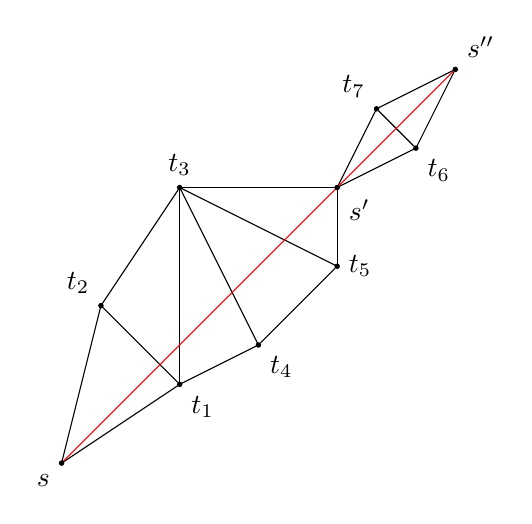
\begin{tikzpicture}[scale=0.5]
		\node[inner sep=0pt, label=below left:\(s\)] (s0) at (0, 0) {};
		\node[inner sep=0pt, label=below right:\(t_1\)] (s1) at (3, 2) {};
		\node[inner sep=0pt, label=above left:\(t_2\)] (s2) at (1, 4) {};
		\node[inner sep=0pt, label=above:\(t_3\)] (s3) at (3, 7) {};
		\node[inner sep=0pt, label=below right:\(t_4\)] (s4) at (5, 3) {};
		\node[inner sep=0pt, label=right:\(t_5\)] (s5) at (7, 5) {};
		\node[inner sep=0pt, label=below right:\(s'\)] (s6) at (7, 7) {};
		\node[inner sep=0pt, label=below right:\(t_6\)] (s7) at (9, 8) {};
		\node[inner sep=0pt, label=above left:\(t_7\)] (s8) at (8, 9) {};
		\node[inner sep=0pt, label=above right:\(s''\)] (s9) at (10, 10) {};

		\draw[color=black] (s0) -- (s1);
		\draw[color=black] (s0) -- (s2);
		\draw[color=black] (s1) -- (s2);
		\draw[color=black] (s1) -- (s3);
		\draw[color=black] (s1) -- (s4);
		\draw[color=black] (s2) -- (s3);
		\draw[color=black] (s3) -- (s4);
		\draw[color=black] (s3) -- (s5);
		\draw[color=black] (s3) -- (s6);
		\draw[color=black] (s4) -- (s5);
		\draw[color=black] (s5) -- (s6);
		\draw[color=black] (s6) -- (s7);
		\draw[color=black] (s6) -- (s8);
		\draw[color=black] (s7) -- (s8);
		\draw[color=black] (s7) -- (s9);
		\draw[color=black] (s8) -- (s9);
		\draw[color=red] (s0) -- (s9);

		\fill[color=black] (s0) circle (2pt);
		\fill[color=black] (s1) circle (2pt);
		\fill[color=black] (s2) circle (2pt);
		\fill[color=black] (s3) circle (2pt);
		\fill[color=black] (s4) circle (2pt);
		\fill[color=black] (s5) circle (2pt);
		\fill[color=black] (s6) circle (2pt);
		\fill[color=black] (s7) circle (2pt);
		\fill[color=black] (s8) circle (2pt);
		\fill[color=black] (s9) circle (2pt);
	\end{tikzpicture}
	\caption{Example unfolded section of a mesh in black with a geodesic between \(s\) and \(s''\) shown in red.}
	\label{fig:geodesic_unfolded_mesh}
\end{figure}

\section{Geodesic Distance}

For this section, due to complexities with the reverse computation, we only have a single variable definition: \begin{center}\begin{tabular}{r|l}
	\(\phi\) & Vector of geodesic distances in \(\mathbb{R}^{\abs{E_G}}\)
\end{tabular}\end{center}

Notation-wise, we will talk about geodesic paths between \(s\) and \(s'\), both in \(E_G\). This actually means we are interested in projecting \(s\) and \(s'\) to the mesh surface, moving them to the nearest mesh vertices, then finding the geodesic path between those two mesh vertices.

\subsection{Forward Computation}
We use \href{https://github.com/zishun/MeshUtility}{MeshUtility}'s implementation of the fast marching method to compute geodesic paths between \(s\) and \(s'\) for every edge \(\cof{s, s'} \in E_G\). This method returns a sequence of vertices and edges the geodesic path passes through, as well as where across the edges the path passes. Automatically, this gives an easy way to compute the geodesic distance.

\subsection{Reverse Computation}
The reverse computation is unfortunately rather complicated and requires some casework. The overall strategy is to first compute the derivative of the geodesic distance between two vertices with respect to the length of any edge in \(E_M\), and then use the chain rule to find the partials we actually want.

To start, a geodesic path is a straight line on an unfolded representation of the mesh, as in Figure~\ref{fig:geodesic_unfolded_mesh}. In fact, we can assign coordinates in \(\mathbb{R}^2\) to the vertices such that the geodesic distance is the Euclidean distance between the start and end points. In the interest of keeping the notation in this section readable, we will use the name of vertices (\(s\), \(t_1\), etc.) to denote these two-dimensional coordinates.

Each geodesic path can be partitioned by the vertices it passes through. If we have the partials of the lengths of each of these segments with respect to each of the mesh's edges, then we automatically have the partials of the length of the entire geodesic simply by addition. In our example, the geodesic path passes through \(s\), \(s'\), and \(s''\). Our analysis below will focus on the segment between \(s\) and \(s'\).

An extremely useful tool is the law of cosines, as well as its derivative. That is, for any three vectors \(u_1\), \(u_2\), and \(u_3\), we have \[\norm{u_2 - u_3}_2^2 = \norm{u_1 - u_2}_2^2 + \norm{u_1 - u_3}_2^2 - 2\pof{u_1 - u_2} \cdot \pof{u_1 - u_3},\] where the last term can be rewritten in terms of the cosine of the angle between \(u_1 - u_2\) and \(u_1 - u_3\).

Define \(M\) to be the length of the distance from \(s\) to \(s'\) (that is, \(M = \norm{s' - s}_2\)), and denote \(\theta_{abc} = m\angle abc\) for any \(a\), \(b\), and \(c\). The partials can be broken into four cases: \begin{itemize}
	\item
	Edges on the boundary. For example, edge \(\cof{t_2, t_3}\). We can then simplify the diagram to Figure~\ref{fig:geodesic_boundary}.

	\begin{figure}[ht]
		\centering
		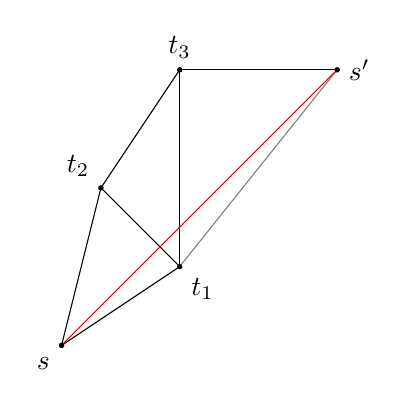
\begin{tikzpicture}[scale=0.5]
			\node[inner sep=0pt, label=below left:\(s\)] (s0) at (0, 0) {};
			\node[inner sep=0pt, label=below right:\(t_1\)] (s1) at (3, 2) {};
			\node[inner sep=0pt, label=above left:\(t_2\)] (s2) at (1, 4) {};
			\node[inner sep=0pt, label=above:\(t_3\)] (s3) at (3, 7) {};
			\node[inner sep=0pt, label=right:\(s'\)] (s6) at (7, 7) {};

			\draw[color=black] (s0) -- (s1);
			\draw[color=black] (s0) -- (s2);
			\draw[color=black] (s1) -- (s2);
			\draw[color=black] (s1) -- (s3);
			\draw[color=gray] (s1) -- (s6);
			\draw[color=black] (s2) -- (s3);
			\draw[color=black] (s3) -- (s6);
			\draw[color=red] (s0) -- (s6);

			\fill[color=black] (s0) circle (2pt);
			\fill[color=black] (s1) circle (2pt);
			\fill[color=black] (s2) circle (2pt);
			\fill[color=black] (s3) circle (2pt);
			\fill[color=black] (s6) circle (2pt);
		\end{tikzpicture}
		\caption{Simplification of Figure~\ref{fig:geodesic_unfolded_mesh} when considering \(\cof{t_2, t_3}\).}
		\label{fig:geodesic_boundary}
	\end{figure}

	Let \(m = \norm{t_2 - t_3}_2\). Applying the law of cosines to \(\angle st_1s'\) and \(\angle t_2t_1t_3\) and differentiating, we have \begin{align*}
		M\frac{\partial M}{\partial m} &= \norm{t_1 - s}_2 \cdot \norm{t_1 - s'}_2 \cdot \sin\pof{\theta_{st_1s'}}\frac{\partial\theta_{st_1s'}}{\partial m}, \\
		m &= \norm{t_1 - t_2}_2 \cdot \norm{t_1 - t_3}_2 \cdot \sin\pof{\theta_{t_2t_1t_3}}\frac{\partial\theta_{t_2t_1t_3}}{\partial m}.
	\end{align*} Now we notice that \(\partial\theta_{st_1s'} / \partial m = \partial\theta_{t_2t_1t_3} / \partial m\), so \[\frac{\partial M}{\partial m} = \frac{\norm{t_2 - t_3}_2 \cdot \norm{\pof{t_1 - s} \times \pof{t_1 - s'}}_2}{\norm{s' - s}_2 \cdot \norm{\pof{t_1 - t_2} \times \pof{t_1 - t_3}}_2}.\]

	\item
	Edges in the interior where the start and end are on ``opposite sides.'' Edge \(\cof{t_1, t_3}\), as shown in Figure~\ref{fig:geodesic_interior_unshared}, exemplifies this case.
	\begin{figure}[ht]
		\centering
		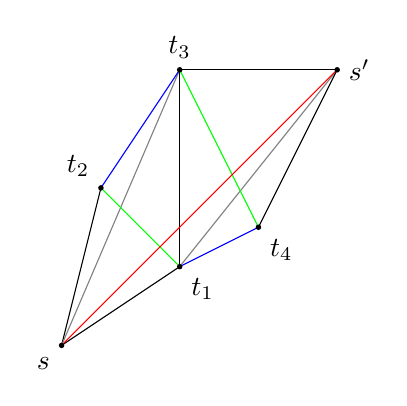
\begin{tikzpicture}[scale=0.5]
			\node[inner sep=0pt, label=below left:\(s\)] (s0) at (0, 0) {};
			\node[inner sep=0pt, label=below right:\(t_1\)] (s1) at (3, 2) {};
			\node[inner sep=0pt, label=above left:\(t_2\)] (s2) at (1, 4) {};
			\node[inner sep=0pt, label=above:\(t_3\)] (s3) at (3, 7) {};
			\node[inner sep=0pt, label=below right:\(t_4\)] (s4) at (5, 3) {};
			\node[inner sep=0pt, label=right:\(s'\)] (s6) at (7, 7) {};

			\draw[color=black] (s0) -- (s1);
			\draw[color=black] (s0) -- (s2);
			\draw[color=gray] (s0) -- (s3);
			\draw[color=green] (s1) -- (s2);
			\draw[color=black] (s1) -- (s3);
			\draw[color=blue] (s1) -- (s4);
			\draw[color=gray] (s1) -- (s6);
			\draw[color=blue] (s2) -- (s3);
			\draw[color=green] (s3) -- (s4);
			\draw[color=black] (s3) -- (s6);
			\draw[color=black] (s4) -- (s6);
			\draw[color=red] (s0) -- (s6);

			\fill[color=black] (s0) circle (2pt);
			\fill[color=black] (s1) circle (2pt);
			\fill[color=black] (s2) circle (2pt);
			\fill[color=black] (s3) circle (2pt);
			\fill[color=black] (s4) circle (2pt);
			\fill[color=black] (s6) circle (2pt);
		\end{tikzpicture}
		\caption{Simplification of Figure~\ref{fig:geodesic_unfolded_mesh} when considering \(\cof{t_1, t_3}\). Note that the triangles \(\triangle st_1t_2\) and \(\triangle s't_3t_4\) are connected to opposite sides of the quadrilateral \(\square t_1t_4t_3t_2\). Alternatively, the two triangles share no vertices.}
		\label{fig:geodesic_interior_unshared}
	\end{figure}

	The computation here is unfortunately complex, but the idea is similar to that of the previous case. Let \(m = \norm{t_1 - t_3}_2\). We first apply the law of cosines to \(\angle t_3t_2t_1\), and \(\angle t_3t_2s\). Then we differentiate each result. This yields \begin{align*}
		\frac{\partial\theta_{t_3t_2t_1}}{\partial m} &= \frac{\norm{t_3 - t_1}_2}{\norm{\pof{t_2 - t_1} \times \pof{t_2 - t_3}}_2}, \\
		\frac{\partial\norm{t_3 - s}_2}{\partial m} &= \frac{\norm{\pof{t_2 - s} \times \pof{t_2 - t_3}}_2}{\norm{t_3 - s}_2} \cdot \frac{\partial\theta_{t_3t_2s}}{\partial m}. \\
		\intertext{Noting that \(\partial\theta_{t_3t_2s} / \partial m\) and \(\partial\theta_{t_3t_2t_1} / \partial m\) are equivalent, we obtain.}
		\frac{\partial\norm{t_3 - s}_2}{\partial m} &= \frac{\norm{t_3 - t_1}_2 \cdot \norm{\pof{t_2 - s} \times \pof{t_2 - t_3}}_2}{\norm{t_3 - s}_2 \cdot \norm{\pof{t_2 - t_1} \times \pof{t_2 - t_3}}_2}. \\
		\intertext{Similarly,}
		\frac{\partial\norm{t_1 - s'}_2}{\partial m} &= \frac{\norm{t_1 - t_3}_2 \cdot \norm{\pof{t_4 - s'} \times \pof{t_4 - t_1}}_2}{\norm{t_1 - s'}_2 \cdot \norm{\pof{t_4 - t_3} \times \pof{t_4 - t_1}}_2}.
	\end{align*}

	Now we apply the law of cosines to \(\angle st_1s'\) and differentiate. This yields \begin{align*}
		\norm{s' - s}_2\frac{\partial M}{\partial m} &= \norm{t_1 - s'}_2 \cdot \frac{\partial\norm{t_1 - s'}_2}{\partial m} - \frac{\pof{t_1 - s} \cdot \pof{t_1 - s'}}{\norm{t_1 - s'}_2} \cdot \frac{\partial\norm{t_1 - s'}_2}{\partial m} \\
		&\qquad + \norm{\pof{t_1 - s} \times \pof{t_1 - s'}}_2 \cdot \frac{\partial\theta_{st_1s'}}{\partial m} \\
		&= \pof{1 - \frac{\pof{t_1 - s} \cdot \pof{t_1 - s'}}{\norm{t_1 - s'}_2^2}} \cdot \frac{\norm{t_1 - t_3}_2 \cdot \norm{\pof{t_4 - s'} \times \pof{t_4 - t_1}}_2}{\norm{\pof{t_4 - t_3} \times \pof{t_4 - t_1}}_2} \\
		&\qquad+ \norm{\pof{t_1 - s} \times \pof{t_1 - s'}}_2 \cdot \frac{\partial\theta_{st_1s'}}{\partial m}. \\
		\intertext{Applying the same process to \(\angle t_1s't_3\), \(\angle s't_3s\), and \(\angle t_3st_1\), we get}
		\norm{t_1 - t_3}_2 &= \pof{1 - \frac{\pof{t_3 - s'} \cdot \pof{t_1 - s'}}{\norm{t_1 - s'}_2^2}} \cdot \frac{\norm{t_1 - t_3}_2 \cdot \norm{\pof{t_4 - s'} \times \pof{t_4 - t_1}}_2}{\norm{\pof{t_4 - t_3} \times \pof{t_4 - t_1}}_2} \\
		&\qquad+ \norm{\pof{t_1 - s'} \times \pof{t_3 - s'}}_2 \cdot \frac{\partial\theta_{t_1s't_3}}{\partial m}, \\
		\norm{s' - s}_2\frac{\partial M}{\partial m} &= \pof{1 - \frac{\pof{t_3 - s} \cdot \pof{t_3 - s'}}{\norm{t_3 - s'}_2^2}} \cdot \frac{\norm{t_1 - t_3}_2 \cdot \norm{\pof{t_2 - s} \times \pof{t_2 - t_3}}_2}{\norm{\pof{t_2 - t_1} \times \pof{t_2 - t_3}}_2} \\
		&\qquad+ \norm{\pof{t_3 - s} \times \pof{t_3 - s'}}_2 \cdot \frac{\partial\theta_{s't_3s}}{\partial m}, \\
		\intertext{and}
		\norm{t_1 - t_3}_2 &= \pof{1 - \frac{\pof{t_1 - s'} \cdot \pof{t_3 - s'}}{\norm{t_3 - s'}_2^2}} \cdot \frac{\norm{t_1 - t_3}_2 \cdot \norm{\pof{t_2 - s} \times \pof{t_2 - t_3}}_2}{\norm{\pof{t_2 - t_1} \times \pof{t_2 - t_3}}_2} \\
		&\qquad+ \norm{\pof{t_1 - s} \times \pof{t_3 - s}}_2 \cdot \frac{\partial\theta_{t_3st_1}}{\partial m}.
	\end{align*}

	We now recognize \begin{align*}
		\frac{\partial\theta_{st_1s'}}{\partial m} + \frac{\partial\theta_{t_1s't_3}}{\partial m} + \frac{\partial\theta_{s't_3s}}{\partial m} + \frac{\partial\theta_{t_3st_1}}{\partial m} &= \frac{\partial}{\partial m}\pof{\theta_{st_1s'} + \theta_{t_1s't_3} + \theta_{s't_3s} + \theta_{t_3st_1}} \\
			&= \frac{\partial}{\partial m}\pof{2\pi} \\
			&= 0.
	\end{align*} We can thus combine the last four law of cosine computations and cancel out all of the unknown derivatives except \(\partial M / \partial m\). The final result is rather complicated expression. Due to formatting issues, it will be presented in two parts: the numerator and denominator of a fraction. The numerator is \begin{align*}
		&\hspace{-2em}\pof{1 - \frac{\pof{t_1 - s} \cdot \pof{t_1 - s'}}{\norm{t_1 - s'}_2^2}} \cdot \frac{\norm{t_1 - t_3}_2 \cdot \norm{\pof{t_4 - s'} \times \pof{t_4 - t_1}}_2}{\norm{\pof{t_4 - t_3} \times \pof{t_4 - t_1}}_2 \cdot \norm{\pof{t_1 - s} \times \pof{t_1 - s'}}_2} \\
		&+ \pof{1 - \frac{\pof{t_3 - s'} \cdot \pof{t_1 - s'}}{\norm{t_1 - s'}_2^2}} \cdot \frac{\norm{t_1 - t_3}_2 \cdot \norm{\pof{t_4 - s'} \times \pof{t_4 - t_1}}_2}{\norm{\pof{t_4 - t_3} \times \pof{t_4 - t_1}}_2 \cdot \norm{\pof{t_1 - s'} \times \pof{t_3 - s'}}_2} \\
		&+ \pof{1 - \frac{\pof{t_3 - s} \cdot \pof{t_3 - s'}}{\norm{t_3 - s'}_2^2}} \cdot \frac{\norm{t_1 - t_3}_2 \cdot \norm{\pof{t_2 - s} \times \pof{t_2 - t_3}}_2}{\norm{\pof{t_2 - t_1} \times \pof{t_2 - t_3}}_2 \cdot \norm{\pof{t_3 - s} \times \pof{t_3 - s'}}_2} \\
		&+ \pof{1 - \frac{\pof{t_1 - s'} \cdot \pof{t_3 - s'}}{\norm{t_3 - s'}_2^2}} \cdot \frac{\norm{t_1 - t_3}_2 \cdot \norm{\pof{t_2 - s} \times \pof{t_2 - t_3}}_2}{\norm{\pof{t_2 - t_1} \times \pof{t_2 - t_3}}_2 \cdot \norm{\pof{t_1 - s} \times \pof{t_3 - s}}_2} \\
		&- \frac{\norm{t_1 - t_3}_2}{\norm{\pof{t_1 - s'} \times \pof{t_3 - s'}}_2} - \frac{\norm{t_1 - t_3}_2}{\norm{\pof{t_1 - s} \times \pof{t_3 - s}}_2}.
	\end{align*} and the denominator is \[\frac{\norm{s' - s}_2}{\norm{\pof{t_1 - s} \times \pof{t_1 - s'}}_2} + \frac{\norm{s' - s}_2}{\norm{\pof{t_3 - s} \times \pof{t_3 - s'}}_2}.\]

	\item
	Edges in the interior where the start and end are on the ``same side.'' In our example, edge \(\cof{t_3, t_4}\) satisfies this, shown in Figure~\ref{fig:geodesic_interior_shared}.

	\begin{figure}[ht]
		\centering
		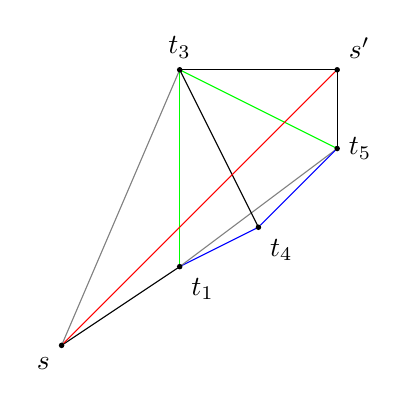
\begin{tikzpicture}[scale=0.5]
			\node[inner sep=0pt, label=below left:\(s\)] (s0) at (0, 0) {};
			\node[inner sep=0pt, label=below right:\(t_1\)] (s1) at (3, 2) {};
			\node[inner sep=0pt, label=above:\(t_3\)] (s3) at (3, 7) {};
			\node[inner sep=0pt, label=below right:\(t_4\)] (s4) at (5, 3) {};
			\node[inner sep=0pt, label=right:\(t_5\)] (s5) at (7, 5) {};
			\node[inner sep=0pt, label=above right:\(s'\)] (s6) at (7, 7) {};

			\draw[color=black] (s0) -- (s1);
			\draw[color=gray] (s0) -- (s3);
			\draw[color=green] (s1) -- (s3);
			\draw[color=blue] (s1) -- (s4);
			\draw[color=gray] (s1) -- (s5);
			\draw[color=black] (s3) -- (s4);
			\draw[color=green] (s3) -- (s5);
			\draw[color=black] (s3) -- (s6);
			\draw[color=blue] (s4) -- (s5);
			\draw[color=black] (s5) -- (s6);
			\draw[color=red] (s0) -- (s6);

			\fill[color=black] (s0) circle (2pt);
			\fill[color=black] (s1) circle (2pt);
			\fill[color=black] (s3) circle (2pt);
			\fill[color=black] (s4) circle (2pt);
			\fill[color=black] (s5) circle (2pt);
			\fill[color=black] (s6) circle (2pt);
		\end{tikzpicture}
		\caption{Simplification of Figure~\ref{fig:geodesic_unfolded_mesh} when considering \(\cof{t_3, t_4}\). Note that the triangles \(\triangle st_1t_3\) and \(\triangle s't_3t_5\) are connected to adjacent sides of the quadrilateral \(\square t_1t_4t_5t_3\). Alternatively, the two triangles share the vertex \(t_3\).}
		\label{fig:geodesic_interior_shared}
	\end{figure}

	Let \(m = \norm{t_3 - t_4}_2\) and \(q = \norm{t_1 - t_5}_2\). Once again, the strategy is to use the law of cosines and differentiate. Using the angles \(\angle t_1t_4t_5\), \(\angle t_4t_5t_3\), \(\angle t_5t_3t_1\), and \(t_3t_1t_4\), we get \begin{align*}
		\norm{t_1 - t_5}_2\frac{\partial q}{\partial m} &= \norm{\pof{t_4 - t_1} \times \pof{t_4 - t_5}}_2 \cdot \frac{\partial\theta_{t_1t_4t_5}}{\partial m}, \\
		\norm{t_3 - t_4}_2 &= \norm{\pof{t_5 - t_3} \times \pof{t_5 - t_4}}_2 \cdot \frac{\partial\theta_{t_4t_5t_3}}{\partial m}, \\
		\norm{t_1 - t_5}_2\frac{\partial q}{\partial m} &= \norm{\pof{t_3 - t_1} \times \pof{t_3 - t_5}}_2 \cdot \frac{\partial\theta_{t_5t_3t_1}}{\partial m}, \\
		\norm{t_3 - t_4}_2 &= \norm{\pof{t_1 - t_3} \times \pof{t_1 - t_4}}_2 \cdot \frac{\partial\theta_{t_3t_1t_4}}{\partial m}.
	\end{align*} We now again apply the trick where the sum of the angle is constant \(2\pi\), meaning the sum of the partials is \(0\). Scaling the equations, adding them, and solving, we get \[\frac{\partial q}{\partial m} = -\frac{\norm{t_3 - t_4}_2 \cdot \pof{\frac{1}{\norm{\pof{t_5 - t_3} \times \pof{t_5 - t_4}}_2} + \frac{1}{\norm{\pof{t_1 - t_3} \times \pof{t_1 - t_4}}_2}}}{\norm{t_1 - t_5}_2 \cdot \pof{\frac{1}{\norm{\pof{t_4 - t_1} \times \pof{t_4 - t_5}}_2} + \frac{1}{\norm{\pof{t_3 - t_1} \times \pof{t_3 - t_5}}_2}}}.\]

	We finish this case by noting \[\frac{\dif M}{\dif q} = \frac{\norm{t_1 - t_5}_2 \cdot \norm{\pof{t_3 - s} \times \pof{t_3 - s'}}_2}{\norm{s - s'}_2 \cdot \norm{\pof{t_3 - t_1} \times \pof{t_3 - t_5}}_2}.\] From the chain rule, we thus have \[\frac{\partial M}{\partial m} = -\frac{\norm{t_3 - t_4}_2 \cdot \norm{\pof{t_3 - s} \times \pof{t_3 - s'}}_2 \cdot \pof{\frac{1}{\norm{\pof{t_5 - t_3} \times \pof{t_5 - t_4}}_2} + \frac{1}{\norm{\pof{t_1 - t_3} \times \pof{t_1 - t_4}}_2}}}{\norm{s - s'}_2 \cdot \pof{\frac{\norm{\pof{t_3 - t_1} \times \pof{t_3 - t_5}}_2}{\norm{\pof{t_4 - t_1} \times \pof{t_4 - t_5}}_2} + 1}}.\]

	\item
	Edges not incident to faces through which the geodesic path passes. The lengths of these edges have no effect on the length of the geodesic path (locally speaking, at least), so the partials here are \(0\).
\end{itemize}

One might think that there is a fifth case missing from the above analysis. In particular, cases similar to that seen in Figure~\ref{fig:geodesic_degenerate} aren't immediately similar to any of the situations referenced above. However, if we make the identifications \begin{align*}
	s &\leftarrow s' & t_1 &\leftarrow s' & t_3 &\leftarrow t_7 \\
	t_4 &\leftarrow t_6 & t_5 &\leftarrow s'' & s' &\leftarrow s'',
\end{align*} we see that Figure~\ref{fig:geodesic_degenerate} is just a degenerate instance of Figure~\ref{fig:geodesic_interior_shared}.

\begin{figure}[ht]
	\centering
	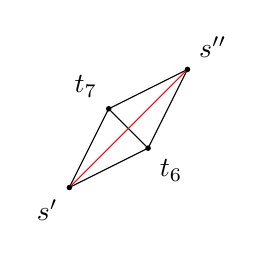
\begin{tikzpicture}[scale=0.5]
		\node[inner sep=0pt, label=below left:\(s'\)] (s6) at (7, 7) {};
		\node[inner sep=0pt, label=below right:\(t_6\)] (s7) at (9, 8) {};
		\node[inner sep=0pt, label=above left:\(t_7\)] (s8) at (8, 9) {};
		\node[inner sep=0pt, label=above right:\(s''\)] (s9) at (10, 10) {};

		\draw[color=black] (s6) -- (s7);
		\draw[color=black] (s6) -- (s8);
		\draw[color=black] (s7) -- (s8);
		\draw[color=black] (s7) -- (s9);
		\draw[color=black] (s8) -- (s9);
		\draw[color=red] (s6) -- (s9);

		\fill[color=black] (s6) circle (2pt);
		\fill[color=black] (s7) circle (2pt);
		\fill[color=black] (s8) circle (2pt);
		\fill[color=black] (s9) circle (2pt);
	\end{tikzpicture}
	\caption{Simplification of Figure~\ref{fig:geodesic_unfolded_mesh} when considering \(\cof{t_6, t_7}\).}
	\label{fig:geodesic_degenerate}
\end{figure}

With the partials of the geodesic distances with respect to the length of the edges of the mesh in hand, we need only compute the partials of the edge lengths with respect to the mesh parameters. We find \[\frac{\partial\norm{v_i - v_j}_2}{\partial z_\ell} = \begin{cases}
	\frac{v_i - v_j}{\norm{v_i - v_j}_2} \cdot \frac{\partial v_\ell}{\partial z_\ell} & \text{if \(\ell = i\),} \\
	\frac{v_j - v_i}{\norm{v_i - v_j}_2} \cdot \frac{\partial v_\ell}{\partial z_\ell} & \text{if \(\ell = j\),} \\
	0 & \text{otherwise.}
\end{cases}\] All that remains is to use the chain rule to compute the partials of the geodesic distance with respect to the mesh parameters.


	% See
% https://libigl.github.io/libigl-python-bindings/tut-chapter1/
% http://multires.caltech.edu/pubs/diffGeoOps.pdf

\subsection{Curvature}
We will define the following: \begin{center}\begin{tabular}{r|l|l}
	\(E_G^\epsilon\) & The set of network edges at threshold \(\epsilon\) & \\ \hline
	\(\kappa^\text{R}_e\) & The Ollivier-Ricci curvature of the edge \(E_G^\epsilon\) & \\ \hline
	\(\widetilde{\kappa^\text{G}}_i\) & The discrete Gaussian curvature at \(v_i\), scaled by vertex area & \(O\pof{\abs{V_M}}\) \\ \hline
	\(\kappa^\text{G}_i\) & The discrete Gaussian curvature at \(v_i\) & \(O\pof{\abs{V_M}}\) \\ \hline
	\(\widetilde{N}_i\) & An outward pointing vector at \(v_i\) & \(O\pof{\abs{V_M}}\) \\ \hline
	\(\widetilde{\kappa^\text{H}}_i\) & The mean curvature normal at \(v_i\) & \(O\pof{\abs{V_M}}\) \\ \hline
	\(\kappa^\text{H}_i\) & The mean curvature at \(v_i\) & \(O\pof{\abs{V_M}}\) \\ \hline
	\(\kappa^+_i\) & The first principal curvature at \(v_i\) & \(O\pof{\abs{V_M}}\) \\ \hline
	\(\kappa^-_i\) & The second principal curvature at \(v_i\) & \(O\pof{\abs{V_M}}\)
\end{tabular}\end{center}

\subsubsection{Ollivier-Ricci Curvature}
We use the GraphRicciCurvature library \cite{ni2019community} to compute the Ollivier-Ricci curvatures of the edges of the graph \(\pof{V_G, E_G^\epsilon}\). Here, \(E_G^\epsilon \subseteq E_G\) is the set of edges whose RTTs are at most \(\epsilon\) milliseconds higher than their GCLs.

Note that \(\kappa^\text{R}_e\) is then only defined for edges in \(E_G^\epsilon\), as opposed to being defined for all edges in \(E_G\). We elide the \(\epsilon\) to reduce notational density.

\subsection{Forward Computation}
For these computations (particularly the mean curvature one), consider \(v\) as a matrix of vertex positions, where each row corresponds to a vertex (so \(v\) is of shape \(\abs{V_M} \times 3\)). We will also use \(e_i\) to denote the \(i\)th standard basis vector. We have \begin{align*}
	\theta_{i, j} &= \arctan\pof{\frac{1}{\cot\pof{\theta_{i, j}}}} \bmod \pi, \\
	\widetilde{\kappa^\text{G}}_i &= 2\pi - \sum_{\substack{k \\ \pof{v_i, v_k} \in E_M}} \theta_{k, c\pof{i, k}}, \\
	\kappa^\text{G} &= D^{-1}\widetilde{\kappa^\text{G}}, \\
	\widetilde{N}_i &= \sum_{\substack{k \\ \pof{v_i, v_k} \in E_M}} N_{i, k}, \\
	\widetilde{\kappa^\text{H}}_i &= -\frac{1}{2}e_i^\intercal D^{-1}L_C^{\text{N}}v, \\
	\kappa^\text{H}_i &= \sgn\pof{\widetilde{N}_i^\intercal\widetilde{\kappa^\text{H}}_i}\norm{\widetilde{\kappa^\text{H}}_i}_2, \\
	\kappa^+_i &= \kappa^{\text{H}}_i + \sqrt{\pof{\kappa^{\text{H}}_i}^2 - \kappa^{\text{G}}_i}, \\
	\kappa^-_i &= \kappa^{\text{H}}_i - \sqrt{\pof{\kappa^{\text{H}}_i}^2 - \kappa^{\text{G}}_i}.
\end{align*}

\subsubsection{Reverse Computation}
Differentiating, \begin{align*}
	\frac{\partial\theta_{i, j}}{\partial z_\ell} &= -\frac{\partial\cot\pof{\theta_{i, j}}}{\partial z_\ell} \cdot \frac{1}{1 + \cot^2\pof{\theta_{i, j}}}, \\
	\frac{\partial\widetilde{\kappa^\text{G}}_i}{\partial z_\ell} &= -\sum_{\substack{k \\ \pof{v_i, v_k} \in E_M}} \frac{\partial\theta_{k, c\pof{i, k}}}{\partial z_\ell}, \\
	\frac{\partial\kappa^\text{G}}{\partial z_\ell} &= D^{-1}\pof{\frac{\dif\widetilde{\kappa^\text{G}}}{\partial z_\ell} - \frac{\dif D}{\partial z_\ell}\kappa^\text{G}}, \\
	\frac{\partial\widetilde{N}_i}{\partial z_\ell} &= \sum_{\substack{k \\ \pof{v_i, v_k} \in E_M}} \frac{\partial N_{i, k}}{\partial z_\ell}, \\
	\frac{\partial\widetilde{\kappa^\text{H}}_i}{\partial z_\ell} &= -\frac{1}{2}e_i^\intercal D^{-1}\pof{\pof{\frac{\partial L_C^{\text{N}}}{\partial z_\ell} - \frac{\partial D}{\partial z_\ell}D^{-1}L_C^{\text{N}}}v + L_C^{\text{N}}\frac{\partial v}{\partial z_\ell}}, \\
	\frac{\partial\kappa_i^\text{H}}{\partial z_\ell} &= \frac{\sgn\pof{\widetilde{N}_i^\intercal\widetilde{\kappa^\text{H}}_i}}{\norm{\widetilde{\kappa^\text{H}}_i}_2}\widetilde{\kappa^\text{H}}_i^\intercal\frac{\partial\widetilde{\kappa^\text{H}}_i}{\partial z_\ell}, \\
	\frac{\partial\kappa^+_i}{\partial z_\ell} &= \frac{2\kappa^+_i\frac{\partial\kappa^{\text{H}}_i}{\partial\rho_i} - \frac{\partial\kappa^{\text{G}}_i}{\partial\rho_i}}{\kappa^+_i - \kappa^-_i}, \\
	\frac{\partial\kappa^-_i}{\partial z_\ell} &= \frac{\frac{\partial\kappa^{\text{G}}_i}{\partial\rho_i} - 2\kappa^-_i\frac{\partial\kappa^{\text{H}}_i}{\partial\rho_i}}{\kappa^+_i - \kappa^-_i}.
\end{align*}


	% \section{Geodesic Loss}

We will define the following in this section: \begin{center}\begin{tabular}{r|l}
	\(t\) & Vector of RTTs in \(\mathbb{R}^{\abs{E_G}}\) \\ \hline
	\(\mathbf{1}\) & Vector of all ones in \(\mathbb{R}^{\abs{E_G}}\) \\ \hline
	\(\nu_0\) & Intermediate value \\ \hline
	\(\nu_1\) & Intermediate value \\ \hline
	\(\delta\) & Intermediate value \\ \hline
	\(\beta_0\) & The constant term in the least squares linear estimator between \(\phi\) and \(t\) \\ \hline
	\(\beta_1\) & The linear term in the least squares linear estimator between \(\phi\) and \(t\) \\ \hline
	\(\mathcal{L}_{\mathrm{geodesic}}\pof{M}\) & The sum of squared residuals when using \(\beta\) as an estimator, scaled to be unitless
\end{tabular}\end{center}

\subsection{Forward Computation}
We make the following computations: \begin{align*}
	\nu_0 &= \pof{\mathbf{1}^\intercal t}\pof{\phi^\intercal\phi} - \pof{t^\intercal\phi}\pof{\mathbf{1}^\intercal\phi}, \\
	\nu_1 &= \abs{E_G}t^\intercal\phi - \pof{\mathbf{1}^\intercal\phi}\pof{\mathbf{1}^\intercal t}, \\
	\delta &= \abs{E_G}\phi^\intercal\phi - \pof{\mathbf{1}^\intercal\phi}^2, \\
	\beta_0 &= \frac{\nu_0}{\delta}, \\
	\beta_1 &= \frac{\nu_1}{\delta}, \\
	\mathcal{L}_{\mathrm{geodesic}}\pof{M} &= \frac{1}{t^\intercal t}\norm{t - \pof{\beta_0\mathbf{1} + \beta_1\phi}}_2^2. \\
\end{align*}

\subsection{Reverse Computation}
The partials of the above quantities are as follows: \begin{align*}
	\frac{\partial\nu_0}{\partial z_\ell} &= \pof{2\pof{\mathbf{1}^\intercal t}\phi - \pof{\mathbf{1}^\intercal\phi}t - \pof{t^\intercal\phi}\mathbf{1}}^\intercal\frac{\partial\phi}{\partial z_\ell}, \\
	\frac{\partial\nu_1}{\partial z_\ell} &= \pof{\abs{E_G} - \pof{\mathbf{1}^\intercal t}\mathbf{1}}^\intercal\frac{\partial\phi}{\partial z_\ell}, \\
	\frac{\partial\delta}{\partial z_\ell} &= 2\abs{E_G}\phi^\intercal\frac{\partial\phi}{\partial z_\ell}, \\
	\frac{\partial\beta_0}{\partial z_\ell} &= \frac{1}{\delta}\pof{\frac{\partial\nu_0}{\partial z_\ell} - \beta_0\frac{\partial\delta}{\partial z_\ell}}, \\
	\frac{\partial\beta_1}{\partial z_\ell} &= \frac{1}{\delta}\pof{\frac{\partial\nu_1}{\partial z_\ell} - \beta_1\frac{\partial\delta}{\partial z_\ell}}, \\
	\frac{\partial\pof{\mathcal{L}_{\mathrm{geodesic}}\pof{M}}}{\partial z_\ell} &= -\frac{2}{t^\intercal t}\pof{t - \pof{\beta_0\mathbf{1} + \beta_1\phi}}\pof{\frac{\partial\beta_1}{\partial z_\ell}\phi + \beta_1\frac{\partial\phi}{\partial z_\ell}}.
\end{align*}


	\subsection{Curvature Loss}

We will define the following: \begin{center}\begin{tabular}{r|l|l}
	\(B_r\pof{e}\) & The ball of radius \(r\) around \(e\) & \(O\pof{\abs{E_G} \cdot \abs{V_M}}\) \\ \hline
	\(\mathcal{L}_{\mathrm{curvature}}\pof{M}\) & Sum of squares of the differences between vertices actual and desired curvatures & \(O\pof{\abs{E_G} \cdot \abs{V_M}}\)
\end{tabular}\end{center} Note that, in practice, the runtimes here will be significantly lower than their upper bounds since balls around edges will not typically contain a large proportion of the mesh's vertices. For example, a square mesh (as described in the main paper) with a relatively small \(\epsilon\) will have the runtimes here be closer to \(O\pof{\abs{E_G}\sqrt{\abs{V_M}}}\).

\subsubsection{Determining the Ball Around an Edge}

Before tackling the loss functional, we must determine what it means for a point to be close to an edge. Suppose \(s\) and \(s'\) are vertices in \(V_G\), and let \(e = \cof{s, s'}\). Recall that \(p_s\) (similarly \(p_{s'}\)) is the point in \(\mathbb{R}^2\) corresponding to \(s\). Define \(\pi\pof{e}\) to be the edge connecting \(p_s\) and \(p_{s'}\). We say that \(v \in B_r\pof{e}\) when \(p_v\) is within distance \(r\) of \(\pi\pof{e}\). Figure~\ref{fig:cuvature_loss_edge_ball} shows this setup.

\begin{figure}[ht]
	\centering
	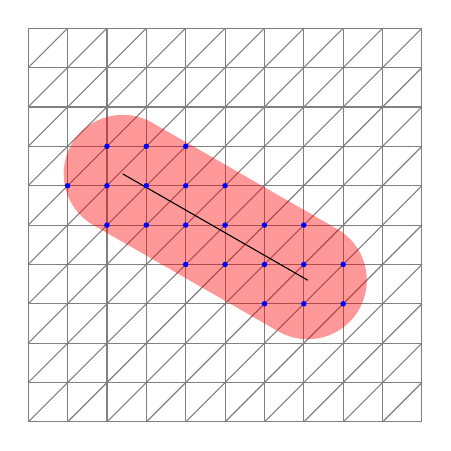
\begin{tikzpicture}[scale=0.5]
		% Draw the mesh
		\foreach \i in {0,...,9}{
			\foreach \j in {0,...,9}{
				\draw[color=gray] (\i,\j)--(\i+1,\j);
				\draw[color=gray] (\i,\j)--(\i,\j+1);
				\draw[color=gray] (\i,\j)--(\i+1,\j+1);
			}
			\draw[color=gray] (\i,10)--(\i+1,10) ;
			\draw[color=gray] (10,\i)--(10,\i+1);
		}

		% Draw the outline of the ball around the edge
		\fill[color=red, opacity=0.4] ({2.4+1.5*cos(atan((7.1-2.4)/(6.3-3.6)))},{6.3+1.5*sin(atan((7.1-2.4)/(6.3-3.6)))}) arc ({atan((7.1-2.4)/(6.3-3.6))}:{atan((7.1-2.4)/(6.3-3.6))+180}:1.5);
		\fill[color=red, opacity=0.4] ({7.1-1.5*cos(atan((7.1-2.4)/(6.3-3.6)))},{3.6-1.5*sin(atan((7.1-2.4)/(6.3-3.6)))}) arc ({atan((7.1-2.4)/(6.3-3.6))-180}:{atan((7.1-2.4)/(6.3-3.6))}:1.5);
		\fill[color=red, opacity=0.4] ({2.4-(1.5*(6.3-3.6)/sqrt((2.4-7.1)^2+(6.3-3.6)^2))},{6.3+(1.5*(2.4-7.1)/sqrt((2.4-7.1)^2+(6.3-3.6)^2))}) -- ({7.1-(1.5*(6.3-3.6)/sqrt((2.4-7.1)^2+(6.3-3.6)^2))},{3.6+(1.5*(2.4-7.1)/sqrt((2.4-7.1)^2+(6.3-3.6)^2))}) -- ({7.1+(1.5*(6.3-3.6)/sqrt((2.4-7.1)^2+(6.3-3.6)^2))},{3.6-(1.5*(2.4-7.1)/sqrt((2.4-7.1)^2+(6.3-3.6)^2))}) -- ({2.4+(1.5*(6.3-3.6)/sqrt((2.4-7.1)^2+(6.3-3.6)^2))},{6.3-(1.5*(2.4-7.1)/sqrt((2.4-7.1)^2+(6.3-3.6)^2))});

		% Draw the edge
		\draw (2.4,6.3)--(7.1,3.6);

		% Draw the points in the ball. Do this manually because automatic is too hard
		\fill[color=blue] (1,6) circle (2pt);
		\fill[color=blue] (2,5) circle (2pt);
		\fill[color=blue] (2,6) circle (2pt);
		\fill[color=blue] (2,7) circle (2pt);
		\fill[color=blue] (3,5) circle (2pt);
		\fill[color=blue] (3,6) circle (2pt);
		\fill[color=blue] (3,7) circle (2pt);
		\fill[color=blue] (4,4) circle (2pt);
		\fill[color=blue] (4,5) circle (2pt);
		\fill[color=blue] (4,6) circle (2pt);
		\fill[color=blue] (4,7) circle (2pt);
		\fill[color=blue] (5,4) circle (2pt);
		\fill[color=blue] (5,5) circle (2pt);
		\fill[color=blue] (5,6) circle (2pt);
		\fill[color=blue] (6,3) circle (2pt);
		\fill[color=blue] (6,4) circle (2pt);
		\fill[color=blue] (6,5) circle (2pt);
		\fill[color=blue] (7,3) circle (2pt);
		\fill[color=blue] (7,4) circle (2pt);
		\fill[color=blue] (7,5) circle (2pt);
		\fill[color=blue] (8,3) circle (2pt);
		\fill[color=blue] (8,4) circle (2pt);
	\end{tikzpicture}
	\caption{An overhead visualization of $B_r\pof{e}$. The mesh is in gray, $\pi\pof{e}$ is in black, and $B_r\pof{e}$ is in blue.}
	\label{fig:cuvature_loss_edge_ball}
\end{figure}

To determine whether a vertex is in the ball, we break the problem into three parts: \begin{itemize}
	\item
	Determine whether \(p_v \in B_r\pof{p_s}\). This is the case when \(\norm{p_v - p_s}_2 < r\).

	\item
	Determine whether the distance from \(p_v\) to \(\pi\pof{e}\) is less than \(r\). To do this, we first project \(p_v\) onto the line containing \(\pi\pof{e}\) to get \(p_{v, e}\): \[p_{v, e} = p_s + \frac{\pof{p_{s'} - p_s}^\intercal\pof{p_v - p_s}}{\norm{p_{s'} - p_s}_2^2}\pof{p_{s'} - p_s}.\] To determine whether this projection lies on the actual segment and that the projection is not too far away from the original point, we simultaneously check the three conditions \begin{align*}
		\pof{p_v - p_s}^\intercal\pof{p_{s'} - p_s} \ge 0, \\
		\pof{p_v - p_{s'}}^\intercal\pof{p_s - p_{s'}} \ge 0, \\
		\norm{p_v - p_{v, e}}_2 < r.
	\end{align*}

	\item
	Determine whether \(p_v \in B_r\pof{p_{s'}}\). This is the case when \(\norm{p_v - p_{s'}}_2 < r\).
\end{itemize} If any of the three above parts yields a positive response, then \(v \in B_r\pof{e}\).

% \subsection[Approximating "Fat Edges" on a Sphere]{Approximating ``Fat Edges''\footnote{This name should really be changed\dots}  on a Sphere}
% For this subsection, we will use notation that has been used elsewhere to mean other things. We do this for readability reasons.

% Consider \(u\), \(v\), and \(r\) all on the unit sphere. Assume that \(u\) and \(v\) are not antipodal. Our goal is to determine whether \(r\) is within a (geodesic) distance of \(\epsilon\) to the shortest arc between \(u\) and \(v\). If this is the case, we write \(r \in B_\epsilon\pof{\pof{u, v}}\).

% We can find the point \(\proj\pof{r}\) nearest to \(r\) on the great circle passing through \(u\) and \(v\) by projecting \(r\) onto the plane spanned by \(u\) and \(v\) and then normalizing the result. The strategy for this is to just use Graham-Schmidt to get an orthonormal basis \(\cof{v, w}\) of the plane. Once we have \(\proj\pof{r}\), we can find the distance from \(r\) to the great circle by taking advantage of the dot product.

% \begin{align*}
% 	\norm{u - \pof{u \cdot v}v}_2^2 &= \norm{u}_2^2 + \pof{u \cdot v}^2\norm{v}_2^2 - 2\pof{u \cdot v}^2 \\
% 		&= 1 + \pof{u \cdot v}^2 - 2\pof{u \cdot v}^2 \\
% 		&= 1 - \pof{u \cdot v}^2, \\
% 	w &\triangleq \frac{u - \pof{u \cdot v}v}{\norm{u - \pof{u \cdot v}v}_2}, \\
% 	\proj\pof{r} &= \frac{\pof{r \cdot v}v + \pof{r \cdot w}w}{\norm{\pof{r \cdot v}v + \pof{r \cdot w}w}_2}, \\
% 	c &\triangleq \norm{\pof{r \cdot v}v + \pof{r \cdot w}w}_2 \\
% 		&= \sqrt{\pof{r \cdot v}^2 + \pof{r \cdot w}^2} \\
% 		&= \sqrt{\pof{r \cdot v}^2 + \pof{r \cdot \frac{u - \pof{u \cdot v}v}{\norm{u - \pof{u \cdot v}v}_2}}^2} \\
% 		&= \sqrt{\pof{r \cdot v}^2 + \frac{\pof{r \cdot u - \pof{r \cdot v}\pof{u \cdot v}}^2}{1 - \pof{u \cdot v}^2}} \\
% 		&= \sqrt{\frac{\pof{r \cdot v}^2 - \pof{r \cdot v}^2\pof{u \cdot v}^2}{1 - \pof{u \cdot v}^2} + \frac{\pof{r \cdot u}^2 + \pof{r \cdot v}^2\pof{u \cdot v}^2 - 2\pof{r \cdot u}\pof{r \cdot v}\pof{u \cdot v}}{1 - \pof{u \cdot v}^2}} \\
% 		&= \sqrt{\frac{\pof{r \cdot u}^2 + \pof{r \cdot v}^2 - 2\pof{r \cdot u}\pof{r \cdot v}\pof{u \cdot v}}{1 - \pof{u \cdot v}^2}} \\
% 	 \cos\pof{\theta} &= r \cdot \proj\pof{r} \\
% 		&= \frac{\pof{r \cdot v}^2 + \pof{r \cdot w}^2}{\norm{\pof{r \cdot v}v + \pof{r \cdot w}w}_2} \\
% 		&= \norm{\pof{r \cdot v}v + \pof{r \cdot w}w}_2 \qquad \text{(by orthonormality)} \\
% 		&= c \\
% 	\theta &= \arccos\pof{c}.
% \end{align*}

% Our real question is whether \(r\) is ``close'' (within distance \(\epsilon\)) to the shortest path from \(u\) to \(v\) on the unit sphere. There are two cases to consider. The first is that \(r\) is very close to \(u\) or \(v\). This can be determined by checking \(\arccos\pof{r \cdot u} < \epsilon\) or \(\arccos\pof{r \cdot v} < \epsilon\) (if either of these is the case, then \(r\) is close).

% The second case is that \(r\) is close to some point that isn't one of the endpoints (this has some overlap with the previous case, but the previous case is easier to check, so we check it first). The trick here is to use the long computation seen above. \(r\) is close to the great circle passing through \(u\) and \(v\) when \[\arccos\pof{c} < \epsilon.\]

% Being a bit more refined, we actually want the angles between \(\proj\pof{r}\) and each of \(u\) and \(v\) to be at most the angle between \(u\) and \(v\). In other words, \begin{align*}
% 	\max\pof{\arccos\pof{\proj\pof{r} \cdot u}, \arccos\pof{\proj\pof{r} \cdot v}} &\le \arccos\pof{u \cdot v} \\
% 	\min\pof{\proj\pof{r} \cdot u, \proj\pof{r} \cdot v} &\ge u \cdot v.
% \end{align*}

% For the left hand side, we can compute
% \begin{align*}
% 	\proj\pof{r} \cdot v &= \frac{\pof{r \cdot v}v + \pof{r \cdot w}w}{\norm{\pof{r \cdot v}v + \pof{r \cdot w}w}_2} \cdot v \\
% 		&= \frac{r \cdot v}{\norm{\pof{r \cdot v}v + \pof{r \cdot w}w}_2} \\
% 		&= \frac{r \cdot v}{c}. \\
% 	\proj\pof{r} \cdot u &= \frac{r \cdot u}{c}. & \text{(by symmetry)}
% \end{align*}

% Putting this together, \(r \in B_\epsilon\pof{\pof{u, v}}\) if and only if one of the following is true:
% \begin{itemize}
% 	\item
% 	\(r \cdot u > \cos\pof{\epsilon}\);
% 	\item
% 	\(r \cdot v > \cos\pof{\epsilon}\);
% 	\item
% 	\(c > \cos\pof{\epsilon}\) and \(\min\pof{r \cdot u, r \cdot v} \ge c\,\pof{u \cdot v}\).
% \end{itemize}

\subsubsection{Forward Computation}
We have \begin{align*}
	\mathcal{L}_{\mathrm{curvature}}\pof{M} &= \frac{1}{\abs{E_G^\epsilon}}\sum_{e \in E_G^\epsilon} \sum_{\substack{k \\ v_k \in B_r\pof{e}}} \pof{\kappa_e^{\text{R}} - \kappa^{\text{G}}_k}^2.
\end{align*}

\subsubsection{Reverse Computation}
Differentiating, \begin{align*}
	\frac{\partial\pof{\mathcal{L}_{\mathrm{curvature}}\pof{M}}}{\partial\rho_\ell} &= \frac{1}{\abs{E_G}}\sum_{e \in E_G} \sum_{\substack{k \\ v_k \in B_\epsilon\pof{e}}} -2\pof{\kappa_e^{\text{R}} - \kappa^G_k}\frac{\partial\kappa^G_k}{\partial z_\ell}.
\end{align*}


	% It would be nice to have something like [SI-MVS](https://www2.eecs.berkeley.edu/Pubs/TechRpts/1993/CSD-93-732.pdf#page=142) (see [this](https://www2.eecs.berkeley.edu/Pubs/TechRpts/1992/CSD-92-664.pdf) too). [Willmore Energy](https://en.wikipedia.org/wiki/Willmore_energy) is another possibility.

% [This](https://www.cad-journal.net/files/vol_4/CAD_4(5)_2007_607-617.pdf) gives a good overview.

\subsection{Smoothness Loss}

We will define the following: \begin{center}\begin{tabular}{r|l|l}
	\(\mathcal{L}_{\mathrm{smooth}}\pof{M}\) & The surface area independent \(\text{MVS}_{\text{cross}}\) energy \cite{Joshi2007EnergyMF} & \(O\pof{\abs{V_M}}\)
\end{tabular}\end{center}

\subsubsection{Forward Computation}
We use \begin{align*}
	\mathcal{L}_{\mathrm{smooth}}\pof{M} &= \pof{-\pof{\kappa^+}^\intercal L_C^{\text{D}}\kappa^+ - \pof{\kappa^-}^\intercal L_C^{\text{D}}\kappa^-} \sum_{\pof{v_i, v_j} \in E_M} A_{i, j}.
\end{align*}

\subsubsection{Reverse Computation}
Differentiating, and using matrix symmetry, \begin{align*}
	\frac{\partial\pof{\mathcal{L}_{\mathrm{smooth}}\pof{M}}}{\partial z_\ell} &= \pof{-\pof{\kappa^+}^\intercal\pof{\frac{\partial L_C^{\text{D}}}{\partial z_\ell}\kappa^+ + 2L_C^{\text{D}}\frac{\partial\kappa^+}{\partial z_\ell}} - \pof{\kappa^-}^\intercal\pof{\frac{\partial L_C^{\text{D}}}{\partial z_\ell}\kappa^- + 2L_C^{\text{D}}\frac{\partial\kappa^-}{\partial z_\ell}}} \sum_{\pof{v_i, v_j} \in E_M} A_{i, j} \\
		&\qquad+ \pof{-\pof{\kappa^+}^\intercal L_C^{\text{D}}\kappa^+ - \pof{\kappa^-}^\intercal L_C^{\text{D}}\kappa^-} \sum_{\pof{v_i, v_j} \in E_M} \frac{\partial A_{i, j}}{\partial z_\ell}.
\end{align*}


	\bibliographystyle{abbrv-doi-hyperref}
	%\bibliographystyle{abbrv-doi-hyperref-narrow}
	%\bibliographystyle{abbrv-doi}
	%\bibliographystyle{abbrv-doi-narrow}

	\bibliography{ref}
\end{document}
